\section{A motivating example: Parkinson's Disease}
\label{intro-complete_ex}

As a motivating example, we now turn to the descriptive
epidemiological meta-regression of Parkinson's Disease (PD). A
systematic review of PD was conducted as part of the GBD 2010
Study.\cite{GBD_2010_or_parkinsons_paper} The results of this review,
data on the prevalence, incidence, and standardized mortality ratio of PD
needed to be combined to produce estimates of disease prevalence by
region, age, sex, and year.  These prevalence estimates were combined
with disability weights to measure Years Lived with Disability (YLDs),
which were then combined with estimates of Years of Life Lost (YLLs)
to produce estimates of the burden of PD quantified in disability
adjusted life-year (DALYs).

PD is a neurodegenerative disorder which includes symptoms of motor
dysfunction, such as tremors, rigidity, and akinesia, in the early
stages of the disease.  As the disease develops, most patients also
develop non-motor symptoms, such as cognitive decline, dementia,
autonomic failure and disordered sleep-wake regulation.  The standard 
definition for PD diagnosis includes at least two of four cardinal 
signs--resting tremor, bradykinesia, rigidity and postural abnormalities.
There is no cure and no known treatments to slow the progression of the disease,
however, motor symptoms and disability may be improved with
symptomatic therapy.\cite{poewe_natural_2006, pollock_prevalence_1966, larsen_clinical_1994}

Systematic review for PD yielded 782 data points total: 660
prevalence, 99 incidence, and 13 standardized mortality ratio data
points that met the inclusion criteria.  The results of a separate
analysis on PD mortality provided an additional $1638$ data points on
the PD cause-specific mortality rate. It is important to note that in
this example, cause-specific mortality means that patients die
\emph{of} the disease and not simply \emph{with} it.  This subtle
distinction is elaborated on in Chapter~\ref{theory-csmr} and
demonstrated further Chapter~\ref{applications-csmr}.  Even when
restricting the data to a specific geographic region, such as Western
Europe, the data remain noisy and heterogeneous, as seen in Figure
\ref{fig:intro-parkinsons data}. This figure shows a horizontal bar
for each data point, where the left and right endpoints depict the
start and end ages of the age interval measured, and the height of the
bar depicts the value of the measurement. Chapters~\ref{theory-age_group_model-overlapping_data}
and~\ref{applications-age_groups} describe our approach to making
robust estimates in the face of such heterogeneous levels and
overlapping age groups.

    \begin{figure}[h]
        \begin{center}
            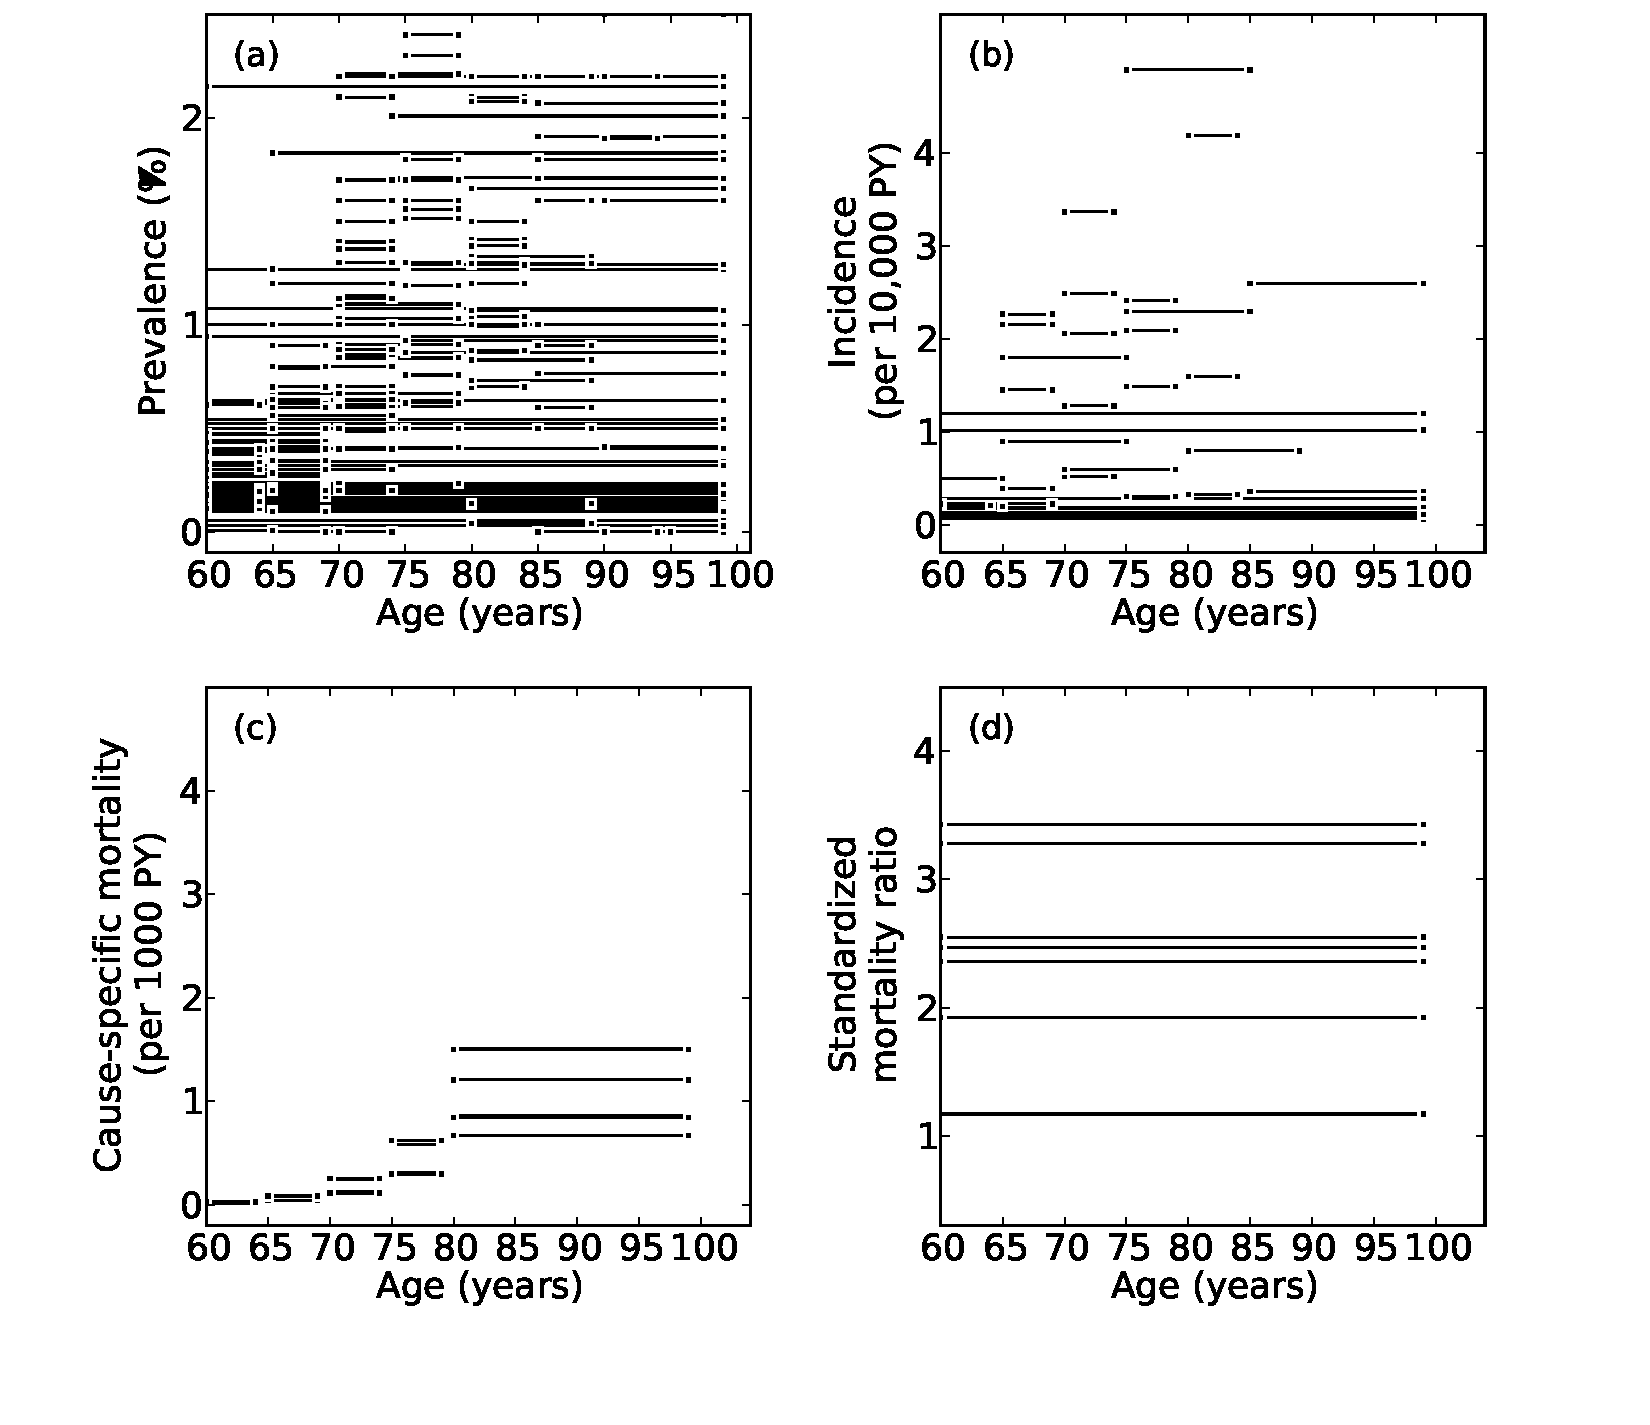
\includegraphics[width=\textwidth]{parkinsons-data.png}
            \caption{Data points from systematic review of descriptive
              epidemiology of Parkinson's Disease, showing data from
              Western Europe on prevalence (panel (a)), incidence
              (panel (b)), cause-specific mortality (panel (c)) and
              the standardized mortality ratio (panel (d)).  Each
              horizontal bar represents one data point collected in
              systematic review, where the left and right endpoints
              represent age range of the heterogeneous age groups, and
              the height of each bar above the $x$-axis represents
              value of measurement.  Each data point also has
              covariate values which are not displayed, as well as a
              standard error, which is also not depicted visually.}
            \label{fig:intro-parkinsons data}
        \end{center}
    \end{figure}

Including data from 1961-2010, the data points represent the results
of many different studies conducted for many different reasons.  Study
level fixed effects, discussed in Chapters \ref{theory-covariate_modeling} and
\ref{applications-efx_study_level}, aid the model in explaining bias
resulting from differing diagnostic criteria and study populations.  Subnational 
studies are shifted by a factor of $e^{-0.03} (e^{-1.1}, e^{1.2})$
compared to nationally-representative studies.  Similarly, studies that 
do not use a neurologist or the standard definition for PD diagnosis are shifted 
by $e^{0.02} (e^{-0.3}, e^{0.3})$ and $e^{-0.48} (e^{-0.7}, e^{-0.2})$,
respectively.

Of the 21 regions reported in the GBD 2010 study, only 36 countries
from 12 regions are represented in the systematic review.  The GBD
2010 study predicts year-age-sex estimates for all countries, even
those without data.  To predict out-of-sample, country level fixed
effects, as described in Chapters \ref{theory-covariate_modeling} and
\ref{applications-efx_country_level}, provide a solution to this
problem of missing epidemiological data.  PD uses smoking prevalence and the 
kilocalories of stimulants consumed per capita per day and national smoking prevalence 
as country level covariates.

Nonsampling variation that cannot be explained is another problem with
such noisy and heterogeneous data.  Chapters
\ref{theory-covariate_modeling} and \ref{applications-rfx} explain how
random effects can be used to detect systematic differences among
different hierarchies of data.

It is intuitive that there is a relationship between these
epidemiological parameters: every prevalent case was once an incident
case, for example.  Combining all parameters to produce internally
consistent results is discussed in detail in Chapter
\ref{sys-dynamics}.  Through the process of data confrontation
discussed in the following chapters, the meta-analysis produces a best
estimate and uncertainty bounds of disease prevalence, as shown in
Figure \ref{fig:intro-parkinsons fit}.

    \begin{figure}[h]
        \begin{center}
            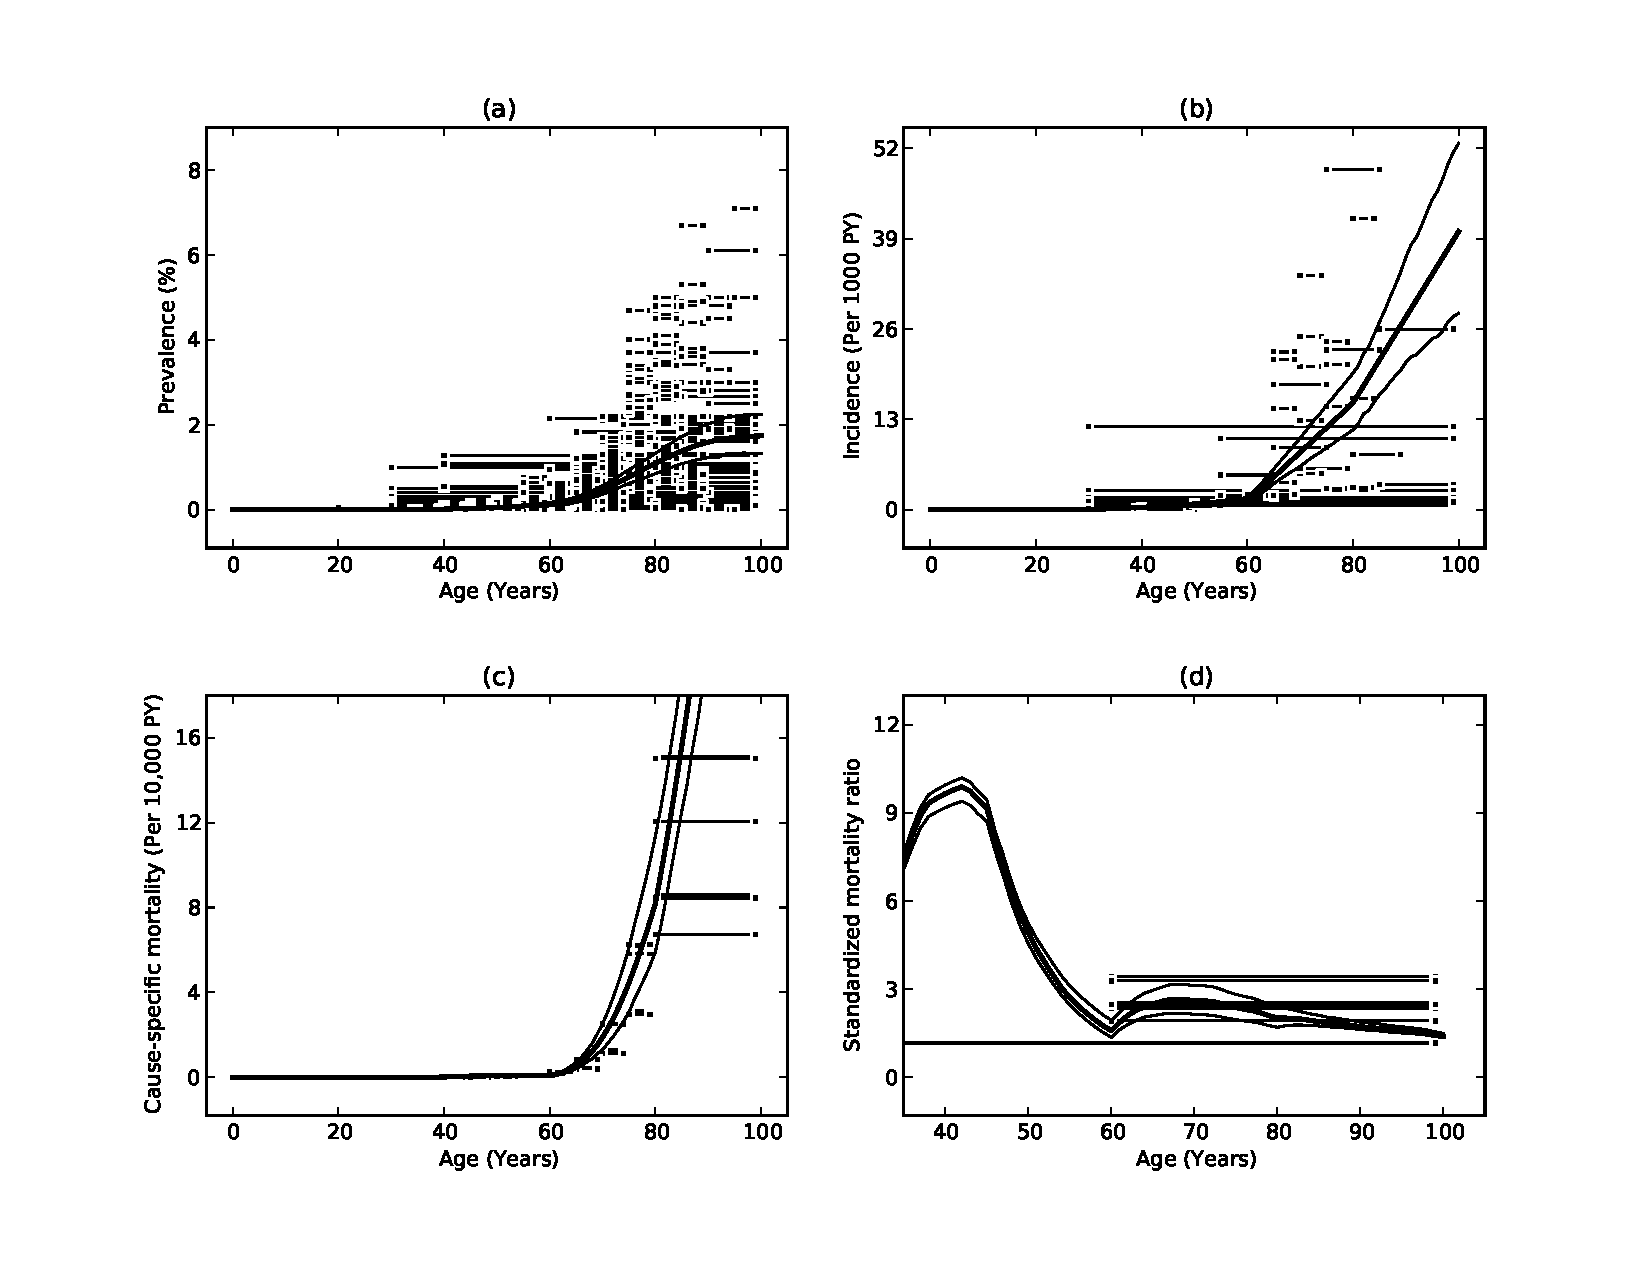
\includegraphics[width=\textwidth]{parkinsons-best.png}
            \caption{Estimates of age-specific rates of
              prevalence (panel (a)), incidence (panel (b)),
              excess mortality (panel (c)) and the
              standardized mortality ratio (panel (d)) of Parkinson's
              disease in Western European females in 2005.}
            \label{fig:intro-parkinsons fit}
        \end{center}
    \end{figure}
